\documentclass[tikz,border=3.14mm]{standalone}
\usepackage{tikz}
\begin{document}

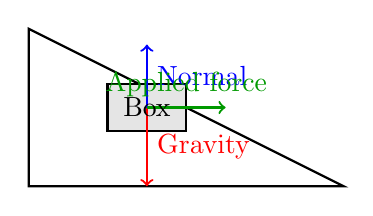
\begin{tikzpicture}
    % Draw the inclined plane
    \draw[thick] (0,0) -- (0,-2) -- (4,-2) -- cycle;

    % Draw the box
    \draw[thick,fill=gray!20] (1,-1.3) rectangle (2,-0.7);

    % Draw the force vectors
    \draw[->,red,thick] (1.5,-1) -- (1.5,-2) node[midway,right] {Gravity};
    \draw[->,blue,thick] (1.5,-1) -- (1.5,-0.2) node[midway,right] {Normal};
    \draw[->,green!60!black,thick] (1.5,-1) -- (2.5,-1) node[midway,above] {Applied force};

    % Label the box
    \node at (1.5, -1) {Box};
\end{tikzpicture}

\end{document}